
\newpage

%\begin{center}
%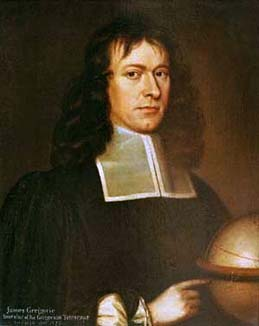
\includegraphics[scale=0.5]{JamesGregory.jpeg}
%\end{center}

\bigskip

\noindent
The fundamental theorem of calculus was established by James Gregory,
a contemporary of Newton.
The theorem is a formal expression of the inverse relation between
integrals and derivatives.
$$\int_a^b f'(x)\,dx=f(b)-f(a)$$
Here is an Eigenmath demonstration of the fundamental theorem of calculus.

\medskip
\verb$f=x^2/2$

\verb$xrange=(-1,1)$

\verb$yrange=xrange$

\verb$draw(d(f))$
% no blank line, otherwise goes to two pages
\begin{center}
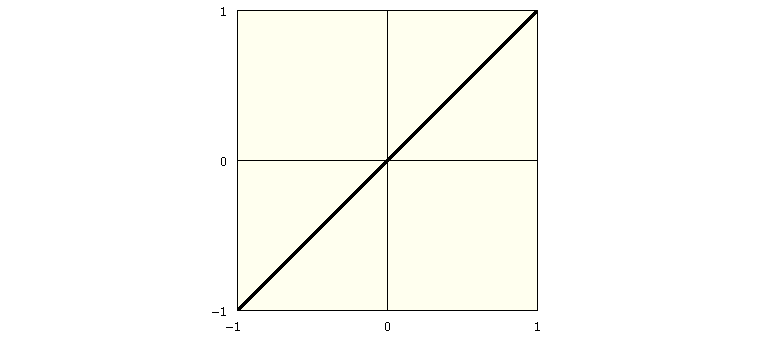
\includegraphics[scale=0.4]{funda1.png}
\end{center}

\verb$draw(integral(d(f)))$

\begin{center}
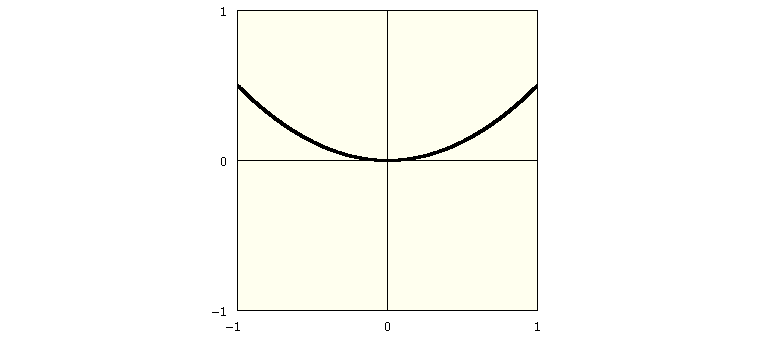
\includegraphics[scale=0.4]{funda2.png}
\end{center}

\noindent
The first graph shows that $f'(x)$ is antisymmetric, therefore the total
area under the curve from $-1$ to $1$ sums to zero.
The second graph shows that $f(1)=f(-1)$.
Hence for $f(x)={1\over2}x^2$ we have
$$\int_{-1}^1f'(x)\,dx=f(1)-f(-1)=0$$

